\documentclass[Report.tex]{subfiles}

\newcommand{\newaxis}[7]{
\begin{axis}[
    ybar,
    title={#1},
    width=#5,
    height=#6,
    ymin=#3, ymax=#4,
    bar width=1em,
    legend style={at={#7},anchor=north,legend columns=-1},
    enlarge x limits=0.4,
    x tick label style={align=center,text width=1.7cm},
    symbolic x coords={Logistic Regression, Random Forest, Multi-layer Perceptron},
    xtick=data,
    ylabel={#2}
]
}


\begin{document}

% #1 - Number of splits
% #2 - Split number
% #3 - Feature name
% #4 - Column name
% #5 - Column legend name
\newcommand{\plotbar}[5]{
\addplot+[
	discard if not={numSplits}{#1},
	discard if not={split}{#2},
	discard if not={features}{#3},
] table [x=model, y=#4,col sep=comma] {data/15-pair-cv.csv};
\addlegendentry{#5}
}

\section{Same player identification}\label{sec:pair-classification}
This sections describes the experiments and analysis of the second question: \textit{Given two matches of Dota 2, is it the same player playing on this hero?}

As the question has changed, some parts of the approach for player identification have changed to adapt to the new question while other parts remained the same. Most notably the input contains features for both matches and the mouse movement features were transformed in order to satisfy this change. 

\subsection{Approach}
%There was a subtle issue with the way the binary classification problem was framed in regards to classifying individual games. This led to high accuracies even with only using mouse movement features, as seen in section \ref{sbsec:game-classification}. The issue had to do with the generality of the model. The models were only trained on a relatively small, fixed set of players, making the problem easier to solve as the models only have to learn the behaviour from the players in the set, which does not apply(TODO) to the general Dota 2 playerbase. Furthermore, the classification is only trained on one particular playing and requires the model to be retrained to be able to predict behaviour of another player. This could be extended into a multi-class problem, but it would still be fixed to the small set of players used in training. This leads to the next machine learning approach of \textit{pair} classification.
%In the next and final approach, deals with this issue by framing the player prediction problem in a different way. Rather than ask \textit{Given a game, which player does it belong to?} the problem is framed as \textit{Given a pair of games, do both games belong to the same player?}
% TODO this leads to low testing accuracies?
% TODO results on a lot more players leads to worse accuracy

The goal of this approach was to be able to train on a large mix of players and games, to learn on features of both matches, and predict if it is the same player, especially if none of the players have been seen by the model before. Instead of learning to match behaviour to specific players, the idea becomes learning the pattern or differences in behaviour between two players. 

In order to train on pairs of matches together, the input features had to be altered to fit as single data points. In the previous experiment, each match was evaluated separately, so every single mouse action in a game could be used and combined, as explained in section \ref{sec:game-approach}. However, in this pair approach, two matches must be used together as the input to a model. Matches in general are of different lengths, which causes the number of mouse actions to be different for every game. Further, the method of generating each mouse movement means even games of the exact same length will not have the same number of actions. The varying number of mouse actions prevents a straightforward use of them as input to a machine learning model. Instead, statistics such as the mean, standard deviation and range must be used. The statistics are calculated for each mouse movement feature over the entire match. For example, the horizontal velocity of a mouse action creates four features, the mean, standard deviation, minimum and maximum horizontal velocity of each \textit{individual} mouse action. There are numerous mouse actions in every match so further statistics of the four statistical features were created, giving new features such as the mean of the mean horizontal velocities. 

Clearly, this approach has many drawbacks. The most obvious is the loss of data from taking averages of averages, as the thousands of mouse actions are reduced to only a small number of statistics. To alleviate this issue as much as possible, the matches can be split into a few portions where each portion has its own statistics. For example, a match can be split into thirds where each third has its own mean, standard deviation and range for each mouse movement feature. Splitting a game this way not only decreases the data loss due to averaging, but enables each portion to be evaluated individually, to see whether any section of a game is more indicative and predictive of player behaviour compared to another section. The drawback with splitting matches like this was the large number of features that end of being created, leading to the curse of dimensionality and excessive computational requirements in extreme cases. Continuing with the horizontal velocity example, TODO

\subsection{Experimental design}
The experimental design for these experiments follow largely from the design described in section \ref{sec:game-experimental} with a few key differences:
\begin{itemize}
\item For mouse movement and game statistic features, each pair of matches could be split into different slices. This creates more features when used together, as a match split into two slices will have double the features, one set for each half of the match. This also allows for comparisons to be made for each slice, to see if any portion of a match is more predictive than another. 
\item 
\end{itemize}

\subsection{Mouse movement features}
%\newcommand{\plotbarmouse11}[2]{
%\plotbar{1}{1}{mouse}{#1}{#2}
%}

TODO mouse movement with different num split

\begin{figure}[H]
\centering
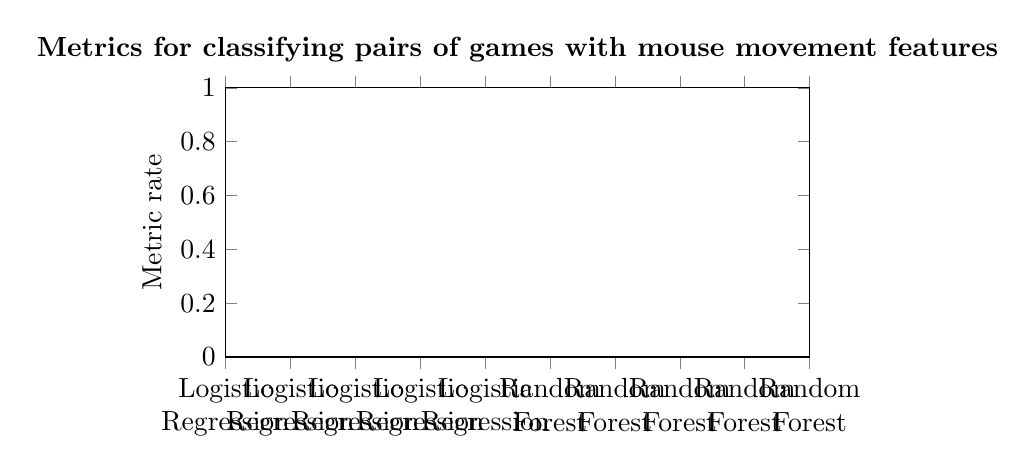
\begin{tikzpicture}
\newaxis{\textbf{Metrics for classifying pairs of games with mouse movement features}}{Metric rate}{0.6}{1.03}{9cm}{5cm}{(0.5,-0.45)}

\plotbar{1}{1}{mouse}{accuracy}{Accuracy}
\plotbar{1}{1}{mouse}{precision}{Precision}
\plotbar{1}{1}{mouse}{recall}{Recall}

\end{axis}
\end{tikzpicture}
\end{figure}

\subsection{Game statistic features}
TODO stats with different num splits

\begin{figure}[H]
\centering
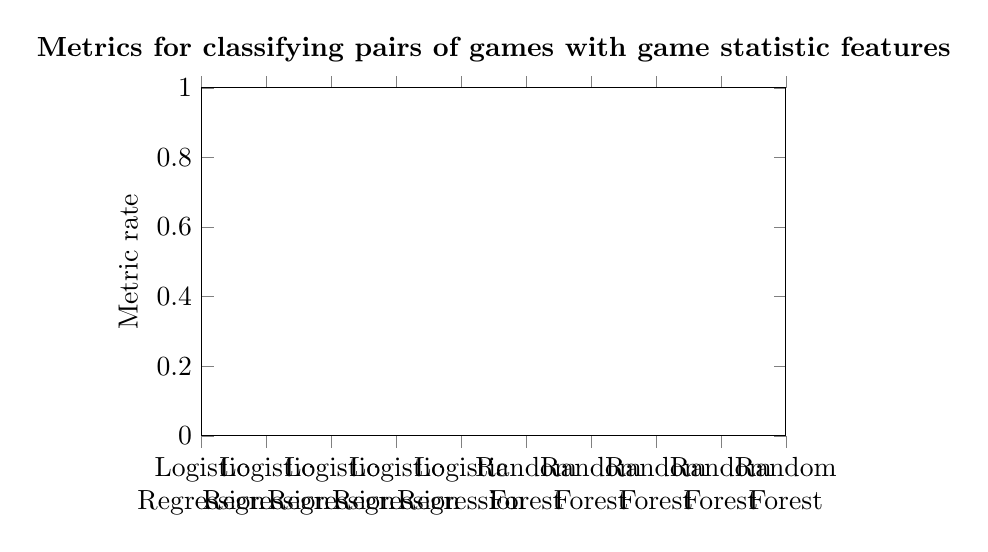
\begin{tikzpicture}
\newaxis{\textbf{Metrics for classifying pairs of games with game statistic features}}{Metric rate}{0.3}{1.03}{9cm}{6cm}{(0.5,-0.35)}

\plotbar{1}{1}{stats}{accuracy}{Accuracy}
\plotbar{1}{1}{stats}{precision}{Precision}
\plotbar{1}{1}{stats}{recall}{Recall}

\end{axis}
\end{tikzpicture}
\end{figure}
\subsection{Itemisation features}
TODO itemisation difference between starting items and end game items for hashed vs one-hot


\begin{figure}[H]
\centering
\begin{subfigure}{1\textwidth}
\centering
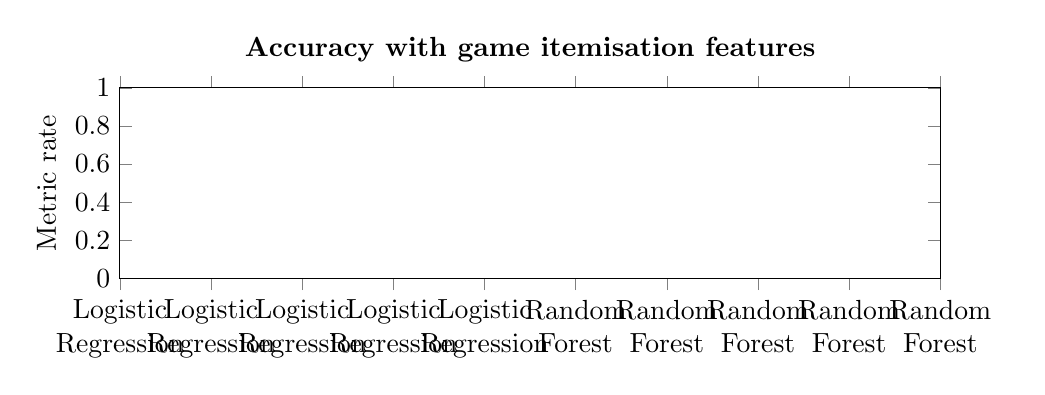
\begin{tikzpicture}
\newaxis{\textbf{Accuracy with game itemisation features}}{Metric rate}{0.75}{1}{12cm}{4cm}{(0.5,-0.65)}

\plotbar{1}{1}{items-hashed}{accuracy}{Hashed items}
\plotbar{1}{1}{items-onehot}{accuracy}{One-hot}
\plotbar{1}{1}{items-starting}{accuracy}{Starting items}
\plotbar{1}{1}{items-select}{accuracy}{Boots only}

\end{axis}
\end{tikzpicture}
\end{subfigure}

\vspace*{1em}
\begin{subfigure}{0.4\textwidth}
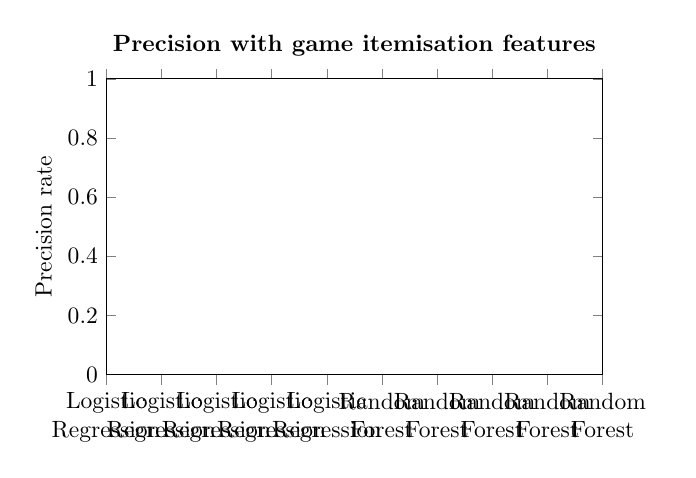
\begin{tikzpicture}[scale=0.85]
\newaxis{\textbf{Precision with game itemisation features}}{Precision rate}{0.75}{1}{9cm}{6cm}{(0.5,-0.25)}

\plotbar{1}{1}{items-hashed}{precision}{Hashed items}
\plotbar{1}{1}{items-onehot}{precision}{One-hot}
\plotbar{1}{1}{items-starting}{precision}{Starting items}
\plotbar{1}{1}{items-select}{precision}{Boots only}
\legend{}; % hide legend

\end{axis}
\end{tikzpicture}
\end{subfigure}
\hspace*{\fill}
\begin{subfigure}{0.4\textwidth}
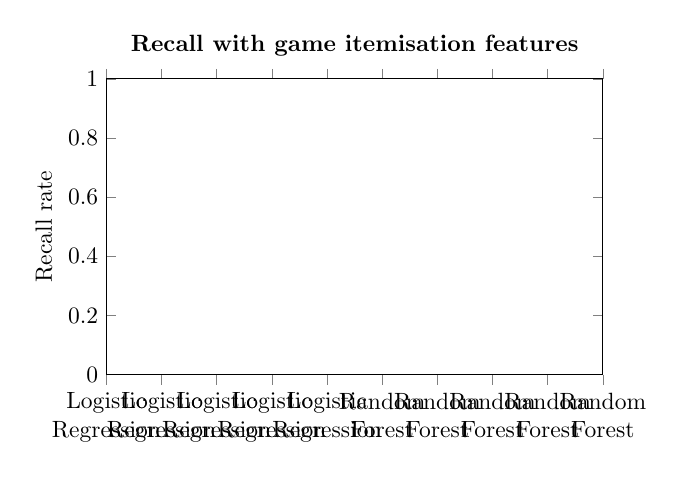
\begin{tikzpicture}[scale=0.85]
\newaxis{\textbf{Recall with game itemisation features}}{Recall rate}{0.75}{1}{9cm}{6cm}{(0.5,-0.25)}

\plotbar{1}{1}{items-hashed}{recall}{Hashed items}
\plotbar{1}{1}{items-onehot}{recall}{One-hot}
\plotbar{1}{1}{items-starting}{recall}{Starting items}
\plotbar{1}{1}{items-select}{recall}{Boots only}
\legend{};

\end{axis}
\end{tikzpicture}
\end{subfigure}
\caption{Accuracy, precision and recall for different game itemisation encoding methods.}
\end{figure}
\subsection{Combined features}

\subsubsection{Comparison of feature individually}
\begin{figure}[H]
\centering
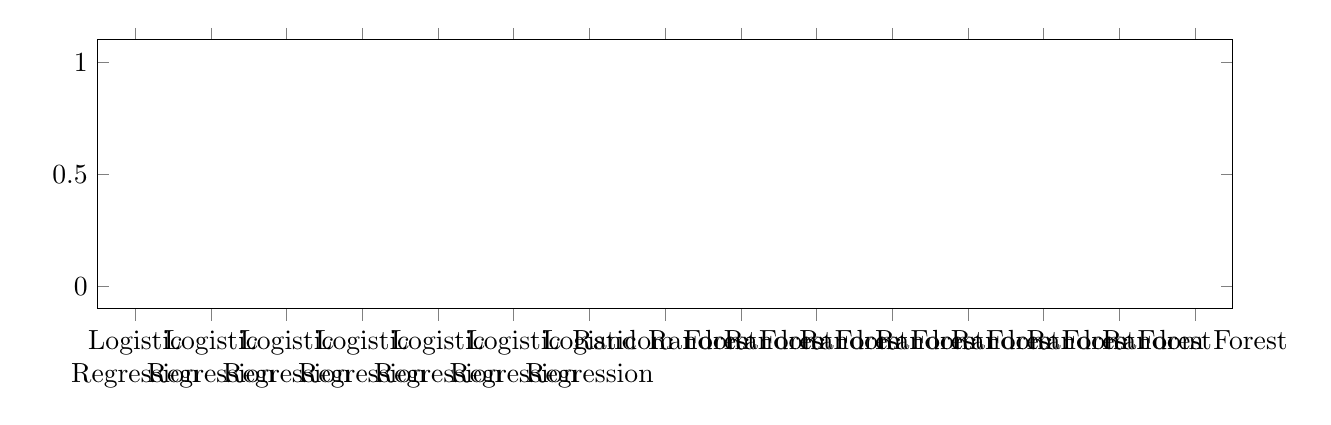
\begin{tikzpicture}
\begin{axis}[
	ybar,
	bar width=1.5em,
	width=16cm,
	height=5cm,
	legend style={at={(0.5,-0.35)},anchor=north,/tikz/every even column/.append style={column sep=0.5cm}},
	xtick=data,
	enlarge x limits=0.25,
	symbolic x coords={Logistic Regression, Random Forest, Multi-layer Perceptron},
    x tick label style={align=center,text width=2.5cm},
]

\plotbar{1}{1}{mouse}{accuracy}{Mouse movement only}
\plotbar{1}{1}{stats}{accuracy}{Game statistics only}
\plotbar{1}{1}{items-onehot}{accuracy}{All items with one-hot encoding}
\plotbar{1}{1}{items-starting}{accuracy}{Starting items only}

\end{axis}
\end{tikzpicture}
\caption{Accuracy for pair classification with different features and models.}
\end{figure}
\subsubsection{Combining best features together}



\end{document}

